\begin{figure}
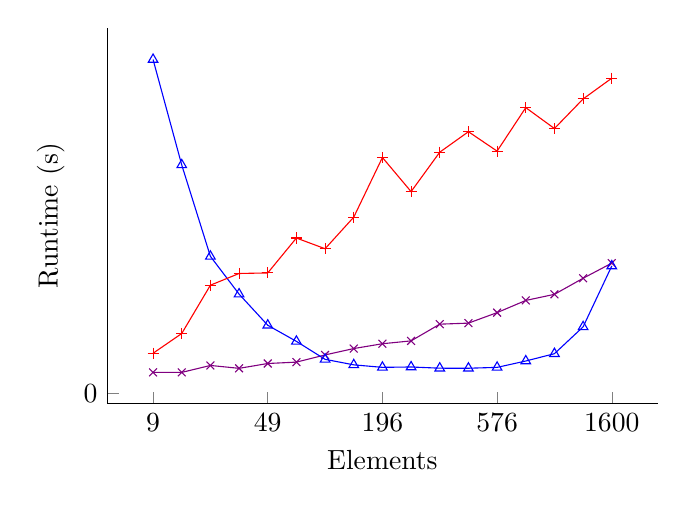
\begin{tikzpicture}
    \begin{axis}[
        height=2.5in,
        width=3.375in,
        axis x line*=bottom,
        axis y line*=left,
        symbolic x coords = {9, 16, 25, 36, 49, 64, 100, 144, 196, 225, 400, 441, 576, 784, 900, 1225, 1600},
        xtick = {9, 49, 196, 576, 1600},
        ytick distance=75,
        domain = 9:1600,
        range = 0:450,
        xlabel={Elements},
        ylabel={Runtime (s)}]
        \addplot[
            mark=x,
            color=violet] coordinates {
                (9, 2.397702)
            	(16, 2.394517) 
            	(25, 3.180994)
            	(36, 2.855465)
            	(49, 3.40153)
            	(64, 3.558418)
            	(100, 4.372501)
            	(144, 5.095191)             	 
            	(196, 5.641578) 
            	(225, 5.964769) 
            	(400, 7.857667) 
            	(441, 7.976037) 
            	(576, 9.166833) 
            	(784, 10.545802) 
            	(900, 11.238055) 
            	(1225, 13.058728)
            	(1600, 14.773929)		
            };                                      
        \addplot[
            mark=triangle,
            color=blue] coordinates {
                (9, 37.839475)
            	(16, 25.899214)
            	(25, 15.539969)
            	(36, 11.263805)
            	(49, 7.735455)
            	(64, 5.908895)
            	(100, 3.875921)
            	(144, 3.248426)             	 
            	(196, 2.967249) 
            	(225, 3.007436) 
            	(400, 2.871237) 
            	(441, 2.866318) 
            	(576, 2.963138) 
            	(784, 3.684828) 
            	(900, 4.5139599) 
            	(1225, 7.553876)
            	(1600, 14.450906)		
            };
        \addplot[
            mark=+,
            color=red] coordinates {
                (9, 4.562236)
            	(16, 6.799783)
            	(25, 12.272318)
            	(36, 13.599193)
            	(49, 13.662346)
            	(64, 17.617201)
            	(100, 16.404489)
            	(144, 19.981687)             	 
            	(196, 26.740117) 
            	(225, 22.875268)
            	(400, 27.343023) 
            	(441, 29.659641) 
            	(576, 27.462272) 
            	(784, 32.388184) 
            	(900, 30.020221) 
            	(1225, 33.37332)
            	(1600, 35.725706)		
            };


    \end{axis}
\end{tikzpicture}
\end{figure}